\chapter{Methodology}
Here we describe the selected algorithms and their parameters in detail. We also discuss the nature of the benchmarks and real world data, giving a summary of the range of tests to be performed. 

\section{Selected Algorithms}
\subsection{Tasgin-Bingol}
One of the earliest implementations of a genetic algorithm for the network clustering problem \cite{Tasgin2006}, Tasgin and Bingol's approach is an example of one of the more naive approaches. Each individual is represented as an array of size $n$, each index corresponding to a node of the input graph. The population is initialized by assigning each gene a random integer, bounded by the number of nodes in the graph. A subset of genes, the size of which is defined by a parameter referred to as the \textit{initialization rate} are selected, and propagate their community assignment to their neighbors. It utilizes modularity as its fitness function. Its mutation operator is simple. For the selected node $i$, select a member of $\Gamma(i)$, and set $i$ to be in its community.

\begin{table}[h!]
	\centering
	\begin{tabular}{|l | r|}
		\hline
		\multicolumn{1}{|c|}{\textbf{Parameter}} & \multicolumn{1}{|c|}{\textbf{Default Value}} \\
		\hline
		\hline
		Population Size & 300 \\
		\hline
		Generations & 30 \\
		\hline
		Elite Portion & 0.10 \\
		\hline
		Mutation Rate  & 0.10 \\
		\hline
		Initialization Rate & 0.60 \\
		\hline
		Cleaning Rate & 0.50 \\
		\hline
		Cleaning Threshold & 0.70 \\
		\hline
		Cleaning Portion & 0.50 \\ [0.2ex] 
		\hline
		
	\end{tabular}
	\caption{Parameters selected as the defaults for our implementation of Tasgin-Bingol's}
	\label{table:tbgadef}
\end{table}
The authors describe a "one-way crossover", to tackle the main issue of the string of groups encoding; The same partition can be represented by multiple chromosomes. The crossover procedure is to randomly select a gene of the first parent, called the \textit{source}. The genes of the parent in this community are then copied to the second parent, the \textit{destination}, who lives on as the offspring.


This can result in disconnected communities, however this is addressed by another operation introduced by the authors, the \textit{cleanup} phase. In chapter 2, the concept of community variance is introduced. During the cleanup phase of the algorithm, some genes are randomly selected from a portion of individuals, and their community variance computed. If the community variance if above a parameter set by the user, that gene is assigned to the community most common to its neighbors.
The algorithm was tested by the authors on limited data, with very high parameters for generations and relatively small population sizes. After achieving results similar to those reported in\cite{Tasgin2006}, we choose to use a much more standard set of default parameters, shown in table \ref{table:tbgadef}.

\subsection{GA-Net}

One of the most widely cited examples of a GA approach to network clustering, GA-Net\cite{Pizzuti2008} 



\subsection{GACD}
\cite{Shi2009}



\subsection{GALS}
GALS\cite{liu2013genetic}


\section{The Girvan-Newman Benchmark}

Girvan and Newman introduce a benchmark which is a special case of the planted $\ell$-partition model\cite{Girvan2002}. The graph is generated by creating 128 nodes, divided into 4 equally sized communities. Each node has an expected degree of 16. By setting the expected $k_{in}$ and $k_{out}$, the difficulty of discerning the partition can be tuned. With an expected $k_{out} < 8$, the communities are strongly defined. It should be expected that a well defined method should discern the structure with a fair degree of accuracy. 

The GN benchmarks limited size makes it an excellent model candidate for testing algorithms in early stages for the ability to detect loosely connected communities, but may not demonstrate the performance of a method when scaled\cite{Yang2016}.


\section{The LFR Benchmark}

\begin{table}[h!]
	\centering
	\begin{tabular}{ |l | l| } 
		\hline
		\multicolumn{1}{|c|}{\textbf{Parameter}} & \multicolumn{1}{|c|}{\textbf{Description}} \\
		\hline
		\hline
		$N$ & Nodes \\ 
		\hline
		$k$ & Average Degree \\ 
		\hline
		$max_k$ & Maximum Degree \\ 
		\hline	
		$mu$ & Mixing Parameter \\ 
		\hline
		$min_c$ & Minimum Community Size \\
		\hline
		$max_c$ & Maximum Community Size \\ 
		\hline
	\end{tabular}
		\caption{The parameters of the LFR benchmark generator}
		\label{table:lfrparams}
\end{table}

\cite{Lancichinetti2008}


\subsubsection{Benchmark Generator}
All synthetic networks were created using Andrea Lancichinetti's benchmark generation applications 

\section{Real World Data}
\subsection{Zachary's Karate Club}
Zachary's Karate Club \cite{Zachary1977} is one of the most widely used networks used to show an algorithm can effectively identify a set of communities. The graph shows the reported relationships between members of a martial arts club, after a schism was formed by a conflict between the lead instructor and the owner of the club. Though small, the graph shows a degree distribution with similar properties to larger examples. Both the instructor and owner are densely connected to the club members who sided with them, with smaller sub-groups forming between members. 

\begin{figure}[!htb]
	\begin{center}
		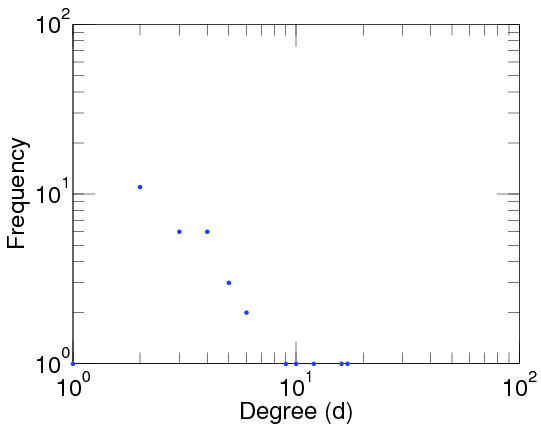
\includegraphics[scale=.4]{images/zachary_degree_dist.png}
	\end{center}
	\caption{Degree distribution of the karate club network\cite{Kunegis2013}}
	\label{logo}
\end{figure}

\subsection{Dolphins}
\cite{Lusseau2003}
\begin{figure}[!htb]
	\begin{center}
		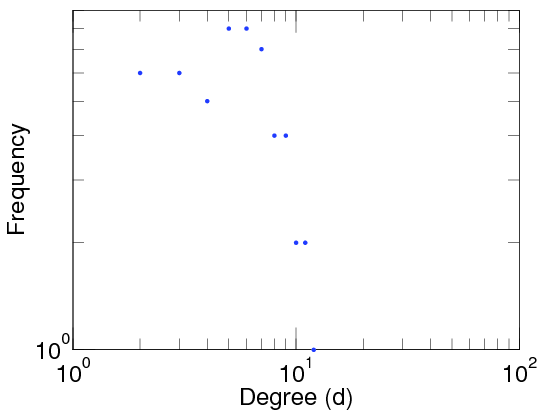
\includegraphics[scale=.4]{images/dolphins_degree_dist.png}
	\end{center}
	\caption{Degree distribution of the Dolphins network\cite{Kunegis2013}}
	\label{logo}
\end{figure}


\subsection{College Football}

\cite{Girvan2002}
\begin{figure}[!htb]
	\begin{center}
		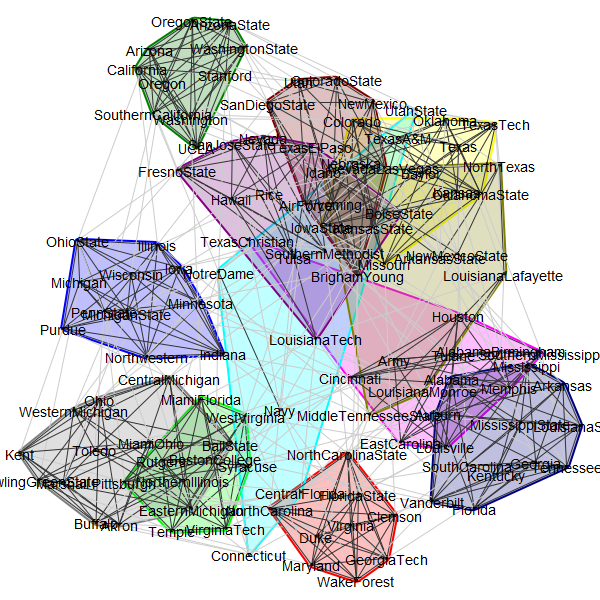
\includegraphics[scale=.4]{images/football.png}
	\end{center}
	\caption{The College Football network, with conferences grouped as communities}
	\label{logo}
\end{figure}


\subsection{Political Blogs}
While the experiments performed have been limited to undirected, unweighted networks, these GA approaches also apply to directed unweighted graphs with little change to the implementation. The Political blogs dataset\cite{Adamic2005} is an observed network, constructed from hyperlinks between blogs focusing on political topics. The data was collected during the course of the United States 2004 federal election campaign. Based on the content of each website, they have been hand labeled as leaning to the left or right of the political spectrum.

The network contains multiple disconnected components of only one node, as well as self-edges, or loops. While a generated network would not assign a single disconnected component a community membership that would be impossible to fulfill, the blogs with no connection to another are still labeled, and will adversely affect the results. For completeness, we present the outputs of both the original network, and a simplified version with no singleton nodes or self edges. 

\begin{figure}
	\begin{tabular}{cc}
		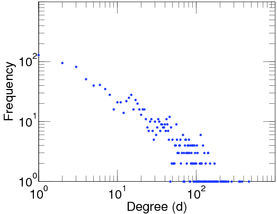
\includegraphics[width=65mm]{images/blogs_total.png} &   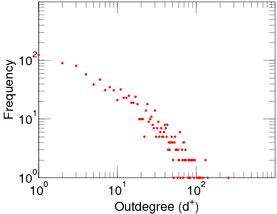
\includegraphics[width=65mm]{images/blogs_out.png} \\
		(a) Total Degree & (b) Outdegree \\[6pt]
		\multicolumn{2}{c}{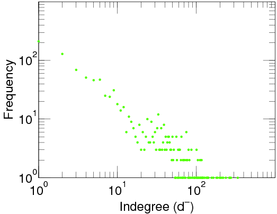
\includegraphics[width=65mm]{images/blogs_in.png} }\\
		\multicolumn{2}{c}{(c) Indegree}
	\end{tabular}
	\caption{The total degree, indegree and outdegree distribution for the political blogs network\cite{Kunegis2013}}
\end{figure}


\section{Clustering Quality Measures}
The goal of this analysis is to compare the performance of the selected algorithms on a sufficient variety of networks, with sufficient complexity. The collection of generated and real world networks has been selected to reflect other comparative studies, and to extend the observations made in the literature proposing the algorithms. These networks come with ground truth, describing the community structure as it was generated, in the case of the synthetic networks, or as it is generally accepted when using real world data.

When comparing the generated community partitions, we use several measures

\subsection{Variation of Information}
\cite{Marina2007}

\subsection{Normalized Mutual Information}
The Normalized Mutual Information (NMI) of a community partition 

\subsection{Rand and Adjusted Rand Index}
\cite{rand1971}


\section{Comparing Performance}

To compare the effectiveness of each algorithm, each experiment is done in two phases. First, each algorithm is run using each of the parameter sets defined. Each parameter set is then compared using a kruskall-wallis test to determine if there is a significant variation in performance. If so, the parameter set yielding the best mean result is used to compare against the other algorithms.